
\chapter{Parity in black-box \textsf{TFNP}} \label{chap:parity-tfnp}

\section{Parity decision trees}

The concept of parity is extensively studied in computer science. In our case, we are interested in exploring parity through the lens of \textit{linear forms modulo 2}, i.e being linear equations defined on $n$ variables over the algebraic field $\F_2$. In this field, each term can either be a 0 or a 1, with the defining characteristic that $1+1 = 0$.

\begin{definition}
    Given $n$ variables $x_1, \ldots, x_n$, we define a \textbf{linear form} as a linear equation over $\F_2$. In general, a linear form can be expressed as $\sum\limits_{i = 1}^n \alpha_i x_i$, where $\alpha_1, \ldots, \alpha_n \in \F_2$
\end{definition}

Intuitively, each sum in a linear form is nothing more than an application of the XOR operator: the linear form $x_1 + x_2$ is equal to 1 if and only if $x_1$ is \textit{different} from $x_2$ (i.e. if $x_1 = 1$ and $x_2 = 0$ or if $x_1 = 0$ and $x_2 = 1$). Additionally, in $\F_2$ the concepts of addition and subtraction are equivalent: since $1+1 = 0$, we easily get that $1 = -1$. Through this properties, parity can be used to determine if two or more objects are equal or not. For example, consider the following system of linear forms:
\[\left \{ \begin{array}{l}
    x_1 + x_2 + x_3 = 1 \\
    x_1 + x_2 + x_4 = 1 \\
    x_1 + x_3 = 1
\end{array} \right .\]

By simplifying the linear system we get that:
\[\left \{ \begin{array}{l}
    x_1 + x_2 + x_3 = 1 \\
    x_1 + x_2 + x_4 = 1 \\
    x_1 + x_3 = 1
\end{array} \right . \longrightarrow
\left \{ \begin{array}{l}
    x_2 = 1\\
    x_1 + 1 + x_4 = 1 \\
    x_1 + x_3 = 1
\end{array} \right . \longrightarrow
\left \{ \begin{array}{l}
    x_2 = 1\\
    x_1 = x_4 \\
    x_1 = 1+x_3
\end{array} \right .\]

which tells us that $x_2 = 1$ and $x_1 = x_4 \neq x_3$ must hold.

\newpage

But what happens if we apply the concept of parity in decision trees? What if, instead of querying variables in order to know their value, we ask the parity of a set of values by querying linear forms? This idea gives rise to the extended model of \textbf{parity decision trees}.

Instead of being labeled by single variables, the nodes of a parity decision tree (PDT for short) are labeled by a linear form $f$. Each node has two outgoing edges, one labeled by $f = 0$ and the other labeled by $f = 1$. Every path from the root of the PDT to one of its nodes defines a system of linear forms given by all the labels of the edges on the path. In general, given the PDT $T$ and a node $v$, we denote this system with $\Phi_v^T$. Given an assignment $\alpha(x_1, \ldots, x_n)$, the output of a PDT is dictated by the parity queries made by each node.

\begin{figure}[H]
    \centering

    \begin{tikzpicture}[->,>=stealth,shorten >=1pt,auto,node distance=1.75cm, thick,main node/.style={scale=0.9,circle,draw,font=\sffamily\normalsize}]

        \node[ellipse, draw] (1)[] {$x_1+x_2+x_3$};

        \node[ellipse, draw] (2) [below left of=1, xshift=-50, ]{$x_1+x_2$};
        \node[ellipse, draw] (3) [below right of=1, xshift=50, ]{$x_1$};

        \node[ellipse, draw] (4) [below left of=2, xshift=-10, ]{$x_2+x_3$};
        \node[ellipse, draw] (5) [below right of=2, xshift=10, ]{$x_2$};
        \node[ellipse, draw] (6) [below left of=3, ]{$x_2$};
        \node[rectangle, draw] (7) [below right of=3]{$o_7$};

        \node[rectangle, draw] (8) [below left of=4, xshift=10, yshift=-10]{$o_1$};
        \node[rectangle, draw] (9) [below right of=4, xshift=-10, yshift=-10]{$o_2$};
        \node[rectangle, draw] (10) [below left of=5, xshift=10, yshift=-10]{$o_3$};
        \node[rectangle, draw] (11) [below right of=5, xshift=-10, yshift=-10]{$o_4$};
        \node[rectangle, draw] (12) [below left of=6, xshift=10, yshift=-10]{$o_5$};
        \node[rectangle, draw] (13) [below right of=6, xshift=-10, yshift=-10]{$o_6$};

        \path[every node/.style={font=\sffamily\small}]
            (1) edge[swap, color=Green]  node{0} (2)
            (1) edge node{1}(3)

            (2) edge[swap]  node{0} (4)
            (2) edge[color=Green]  node{1}(5)

            (3) edge[swap]  node{0} (6)
            (3) edge  node{1}(7)
            
            (4) edge[swap]  node{0} (8)
            (4) edge  node{1}(9)

            (5) edge[swap]  node{0} (10)
            (5) edge[color=Green]  node{1}(11)

            (6) edge[swap]  node{0} (12)
            (6) edge  node{1}(13)
        ;
    \end{tikzpicture}

    \caption{An example of parity decision tree of size 13 and depth 3.}
\end{figure}

In the above example, the green path defines the following system of linear forms:
\[\left \{ \begin{array}{l}
    x_1 + x_2 + x_3 = 0 \\
    x_1 + x_2 = 1 \\
    x_2 = 1
\end{array}\right .\]

which once simplified corresponds to the assignment $x_0 = 0, x_2 = 1, x_3 = 1$. We define the class $\mathsf{FP}^{pdt}$ as the set of $\mathsf{TFNP}^{dt}$ problems that are efficiently solvable by a PDT.

\begin{definition}
    We define $\mathsf{FP}^{pdt}$ as the set of query search problems $R = (R_n)_{n \in \N}$ for which there exists a polylogarithmic depth PDT $T_n$ such that $T_n(x) = y$ if and only if $(x,y) \in R_n$.
\end{definition}

It's easy to see that $\mathsf{FP}^{dt} \subseteq \mathsf{FP}^{pdt}$ since any decision tree is just a PDT with all the queries defined only on one variable. Any PDT can be converted into a normal decision tree simply by "splitting" each linear query. Given a node $v$ labeled with the linear form $f + x_i$, let $u$ and $w$ be the children of $v$ respectively given by $f + x_i = 0$ and $f+x_i = 1$. Let $T_u$ and $T_w$ be the two subtrees with root $u$ and $w$.

\newpage

\begin{figure}[H]
    \centering

    \begin{tikzpicture}[->,>=stealth,shorten >=1pt,auto,node distance=1.75cm, thick,main node/.style={scale=0.9,circle,draw,font=\sffamily\normalsize}]

        \node[ellipse, draw] (1)[] {$f + x_i$};

        \node[circle, draw] (2) [below left of=1, xshift=-50, ]{};
        \node[circle, draw] (3) [below right of=1, xshift=50, ]{};

        \node[] (2a) [below left of=2, yshift=-40]{};
        \node[] (2b) [below right of=2, yshift=-40]{};
        \node[] (2c) [below of=2]{$T_u$};

        \node[] (3a) [below left of=3, yshift=-40]{};
        \node[] (3b) [below right of=3, yshift=-40]{};
        \node[] (3c) [below of=3]{$T_w$};

        \path[every node/.style={font=\sffamily\small}]
            (1) edge[swap]  node{0} (2)
            (1) edge node{1}(3)
        ;

        \path[every node/.style={font=\sffamily\small}, -]
            (2) edge (2a.center)
            (2) edge (2b.center)
            (2a.center) edge (2b.center)
        ;

        \path[every node/.style={font=\sffamily\small}, -]
            (3) edge (3a.center)
            (3) edge (3b.center)
            (3a.center) edge (3b.center)
        ;
    \end{tikzpicture}

    \caption{The initial subtree of a parity decision tree}
\end{figure}

We replace $v$ with the node $v'$ labeled with the linear form $x_i$ and introduce two new nodes $u', w'$ such that $u'$ is the child of $v'$ when $x_i = 0$ and $w'$ is the child of $v'$ when $x_i = 1$. We label $u'$ with the linear form $f$ and let a copy of $T_u$ be the children of $u'$ when $f = 0$, while a copy of $T_w$ is the children of $u'$ when $f = 1$. Symmetrically, we label $w'$ with the linear form $f$ and let a copy of $T_w$ be the children of $w'$ when $f = 0$, while a copy of $T_u$ is the children of $w'$ when $f = 1$. 

\begin{figure}[H]
    \centering

    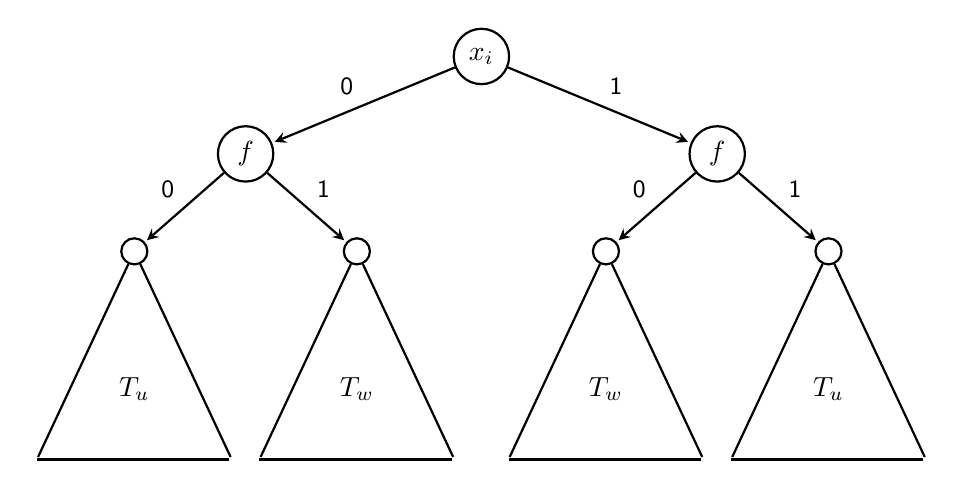
\begin{tikzpicture}[->,>=stealth,shorten >=1pt,auto,node distance=1.75cm, thick,main node/.style={scale=0.9,circle,draw,font=\sffamily\normalsize}]

        \node[circle, draw] (1)[] {$x_i$};

        \node[circle, draw] (2) [below left of=1, xshift=-50, ]{$f$};
        \node[circle, draw] (3) [below right of=1, xshift=50, ]{$f$};

        \node[circle, draw] (2x) [below left of=2, xshift=-5]{};
        \node[circle, draw] (2y) [below right of=2, xshift=5]{};

        \node[circle, draw] (3x) [below left of=3, xshift=-5]{};
        \node[circle, draw] (3y) [below right of=3, xshift=5]{};

        \node[] (2a) [below left of=2x, yshift=-40]{};
        \node[] (2b) [below right of=2x, yshift=-40]{};
        \node[] (2c) [below of=2x]{$T_u$};

        \node[] (3a) [below left of=2y, yshift=-40]{};
        \node[] (3b) [below right of=2y, yshift=-40]{};
        \node[] (3c) [below of=2y]{$T_w$};

        \node[] (4a) [below left of=3x, yshift=-40]{};
        \node[] (4b) [below right of=3x, yshift=-40]{};
        \node[] (4c) [below of=3x]{$T_w$};

        \node[] (5a) [below left of=3y, yshift=-40]{};
        \node[] (5b) [below right of=3y, yshift=-40]{};
        \node[] (5c) [below of=3y]{$T_u$};

        \path[every node/.style={font=\sffamily\small}]
            (1) edge[swap]  node{0} (2)
            (1) edge node{1}(3)

            (2) edge[swap]  node{0} (2x)
            (2) edge node{1}(2y)

            (3) edge[swap]  node{0} (3x)
            (3) edge node{1}(3y)
        ;

        \path[every node/.style={font=\sffamily\small}, -]
            (2x) edge (2a.center)
            (2x) edge (2b.center)
            (2a.center) edge (2b.center)
        ;

        \path[every node/.style={font=\sffamily\small}, -]
            (2y) edge (3a.center)
            (2y) edge (3b.center)
            (3a.center) edge (3b.center)
        ;

        \path[every node/.style={font=\sffamily\small}, -]
            (3x) edge (4a.center)
            (3x) edge (4b.center)
            (4a.center) edge (4b.center)
        ;

        \path[every node/.style={font=\sffamily\small}, -]
            (3y) edge (5a.center)
            (3y) edge (5b.center)
            (5a.center) edge (5b.center)
        ;
    \end{tikzpicture}

    \caption{The subtree after the splitting process}
\end{figure}

By repeating this process until all queries are defined on a single variable, we obtain a decision tree equivalent to the original PDT. This final decision tree has exponential size and polynomial depth, which \textit{may not} be the smallest possible decision tree that solves the search problem solved by the initial PDT. However, we can easily prove that parity decision trees are indeed much stronger than decision trees.

\begin{proposition}
    $\mathsf{FP}^{dt} \subsetneq \mathsf{FP}^{pdt}$
\end{proposition}

\begin{proof}
    Consider the search problem of determining the parity of $n$ variables for a given assignment $\alpha$. This problem can be solved by a PDT that makes single query on all $n$ variables. By applying the splitting process on such tree, we get a decision tree of size $2^n$ and depth $n$. It's easy to see that the resulting decision tree is the smallest possible tree that can solve this search problem.
\end{proof}

\newpage

Since a system of linear forms can have multiple solutions, many assignments could be mapped to the same output. However, some systems could also be unsatisfiable, meaning that the node cannot is unreachable by any assignment. When this happens we say that the node is \textbf{degenerate}.

Like normal decision trees, PDTs can be used to solve the false clause search problem associated with any unsatisfiable CNF. A parity decision tree for a CNF formula $F$ is a PDT defined on the same variables of $F$ where for each leaf $v$ one of the following conditions holds:
\begin{enumerate}[itemsep=0em]
    \item The leaf is \textit{degenerate}
    \item The leaf \textit{refutes} a clause $C$ of $F$, meaning that the system $\Phi_v^T$ is satisfiable and every one of its solutions falsifies $C$
    \item The leaf \textit{satisfies} a clause $C$ of $F$, meaning that the system $\Phi_v^T$ has only one solution and it also satisfies $C$
\end{enumerate}

\begin{figure}[H]
    \centering

    \begin{tikzpicture}[->,>=stealth,shorten >=1pt,auto,node distance=1.75cm, thick,main node/.style={scale=0.9,circle,draw,font=\sffamily\normalsize}]

        \node[ellipse, draw] (1)[] {$x + y$};

        \node[ellipse, draw] (2) [below left of=1, xshift=-20, ]{$x$};
        \node[ellipse, draw] (3) [below right of=1, xshift=20, ]{$x$};

        \node[rectangle, draw] (4) [below left of=2, xshift=10, yshift=-10]{$x \lor y$};
        \node[rectangle, draw] (5) [below right of=2, xshift=-10, yshift=-10]{$\lnot x \lor \lnot y$};
        \node[rectangle, draw] (6) [below left of=3, xshift=10, yshift=-10]{$x \lor \lnot y$};
        \node[rectangle, draw] (7) [below right of=3, xshift=-10, yshift=-10]{$\lnot x \lor y$};

        \path[every node/.style={font=\sffamily\small}]
            (1) edge[swap]  node{0} (2)
            (1) edge node{1}(3)

            (2) edge[swap]  node{0} (4)
            (2) edge[]  node{1}(5)

            (3) edge[swap]  node{0} (6)
            (3) edge  node{1}(7)
            
        ;
    \end{tikzpicture}

    \caption{A parity decision tree for $(x \lor y) \land (\lnot x \lor \lnot y) \land (\lnot x \lor y) \land (x \lor \lnot y)$}
\end{figure}

We observe that if a node doesn't meet any of the previous conditions then it cannot be a leaf node. Moreover, we also observe that the system associated with the root of any PDT is always satisfiable due to it containing no linear forms. Since we are interested in studying PDTs for refusing unsatisfiable CNF formulas, the third case will never be true for any leaf. However, we still need a way to exclude the first case since an unsatisfiable system cannot be associated with any assignment. Luckily, each degenerate PDT can be conveniently converted into a non-degenerate one through a very simple process \cite{res_lin_2}.

\begin{proposition}
    \label{degenerate}
    Let $F$ be an unsatisfiable CNF formula. If $S_F$ can be solved with a degenerate PDT of size $s$ and depth $d$, it can also be solved with a non-degenerate PDT of size at most $s$ and depth at most $d$.
\end{proposition}

\begin{proof}
    
    Let $T$ be a degenerate PDT of size $s$ and depth $d$ that solves $S_F$. Let $U$ be the set of degenerate nodes of $T$. Notice that since $\Phi_r^T$ is empty, thus always satisfiable, we know that $r \notin U$. Consider the node $u \in U$ with the minimal distance from the root $r$. Since $u$ is not the root of $T$, there must be two vertices $p$ and $s$ such that $p$ is the parent of $u$ and $s$ is the sibling of $u$.

    We notice that $\Phi_s^T$ must be satisfiable: if we assume that this is not true then both $\Phi_s^T$ and $\Phi_u^T$ would be unsatisfiable, which can be true only if $\Phi_p^T$ is also unsatisfiable, but we chose $w$ as the node in $U$ with minimal distance. Since $\Phi_s^T$ is satisfiable, the label $f = \alpha$ on the edge $(p,s)$ must be already contained inside the system $\Phi_p^T$, meaning that each assignment that satisfies $\Phi_p^T$ also satisfies $\Phi_s^T$.

    We construct a new PDT $T'$ by removing the subtree $T_u$ with root $u$ from the initial PDT $T$ and by contracting the edge $(p,s)$, merging the two the nodes $p$ and $s$ into a single node $v$. In other words, the subtree $T_u$ gets removed and the children of $s$ become the new children of $p$. Each assignment that satisfies $\Phi_p^T$ also satisfies $\Phi_v^{T'}$, concluding that $T'$ also solves $S_F$. By repeating the process until $U$ is empty, we get a non-degenerate PDT that solves $S_F$ of size at most $s$ and depth at most $d$.
\end{proof}

\section{Linear resolution over $\F_2$}

Once we have defined the class $\mathsf{FP}^{pdt}$, we are interested in finding a proof system that characterizes it. Consider a system $\Phi$ of linear forms defined on $\F_2$. This system can be viewed as the conjunction of the linear forms that it describes:
\[\left \{ \begin{array}{c}
    f_1 = \alpha_1 \\
    f_2 = \alpha_2 \\
    \vdots \\
    f_k = \alpha_k
\end{array}\right . \iff (f_1 = \alpha_1) \land (f_2 = \alpha_2) \land \ldots \land (f_k = \alpha_k)\]

We can rewrite these conjunctions as a negation of a disjunction:
\[\bigwedge_{i = 1}^k (f_i = \alpha_i) \iff \lnot \bigvee_{i = 1}^k \lnot (f_i = \alpha_i) \iff \lnot \bigvee_{i = 1}^k (f_i = 1 + \alpha_i)\]

which implies that the negation of the system is equivalent to a set of disjunctions:
\[\lnot \bigwedge_{i = 0}^k (f_1 = \alpha_1) \iff \bigvee_{i = 0}^k (f_1 = 1 + \alpha_1)\]

We say that such set of disjunction is a \textbf{linear clause}. More generally, a \textit{linear CNF formula} over $\F_n$ is a conjunction of linear clauses defined on $\F_n$.

\begin{definition}
    A linear CNF formula is a conjunction of $m$ disjunctions of linear equations over $\F_n$.
    \[\bigwedge_{i = 1}^m \bigvee_{j = 1}^{k_i} (f_j = \alpha_j)\]
\end{definition}

Linear CNF formulas can assume a complex structure such as the following:
\[((x_1+x_2 = 0) \lor (x_1 = 1)) \land ((x_2 + x_3 + x_4 = 3) \lor (x_2 + x_4 = 0))\]

\newpage

We define \textbf{linear Resolution over $\F_n$} (or $\mathsf{ResLin(\F_n)}$), an extension of standard Resolution (see \Cref{chap:bb-tfnp}) based on the following two rules:
\begin{enumerate}
    \item \textit{Resolution rule}: given two linear clauses $(f = 0) \lor C$ and $(f = 1) \lor D$ defined on $\F_n$, we can derive the linear clause $C \lor D$
    \item \textit{Weakening rule}: given a linear clause $C$, we can derive any linear clause $D$ such that $C \implies D$.
\end{enumerate}

Like in normal resolution, in $\mathsf{ResLin(\F_n)}$ any derivation of a linear clause $C$ from a linear CNF $F$ is a sequence of linear clauses that ends with $C$, where every clause is either an axiom of $F$ or it can be derived from previous clauses through one of the two derivation rules. A linear CNF is unsatisfiable if and only if the empty linear clause can be derived from it. Furthermore, each clause in a derivation is used at most once we say that the derivation has a \textit{tree-like} structure.

Any standard CNF formula can be described as a linear CNF formula over $\F_2$ simply by treating each clause as a disjunction of linear forms made of a single term. For example, the CNF $(x_1 \lor \lnot{x_2}) \land (\lnot{x_3} + x_1)$ can be written as the following linear CNF formula:
\[((x_1 = 1) \lor (x_2 = 0)) \land ((x_3 = 0) \lor (x_1 = 1))\]

We call this the \textit{linear encoding} of a CNF. From now on, we will restrict our interests to linear resolution over $\F_2$, also called \textit{parity resolution} (or $\mathsf{Res}_\oplus$).

The weakening rule makes this proof system powerful thanks to how semantical implications can be used as "shortcuts". For example, consider the following linear CNF:
\[(x = 1) \land (x+y = 1) \land ((x = 0) \lor (y = 1))\]

By rewriting the last linear clause as negation of a conjunction, we notice that:
\[(x = 0) \lor (y = 1) \equiv \lnot ((x = 1) \land (y = 0))\]

By simple substitution we get that:
\[\lnot ((x = 1) \land (y = 0)) \implies  \lnot ((x = 1) \land (x+y = 1))\]

which is equivalent to:
\[\lnot ((x = 1) \land (x+y = 1)) \equiv  (x = 0) \lor (x+y = 0)\]

concluding that $(x = 0) \lor (y = 1) \models (x = 0) \lor (x+y = 0)$. Proceeding with the resolution rule, we get the following tree-like refutation:
\begin{figure}[H]
    \centering
    
    \begin{tikzpicture}[-,>=stealth,shorten >=1pt,auto,node distance=2.25cm, thick,main node/.style={scale=0.9,circle,draw,font=\sffamily\normalsize}]
    
        \node (1) []{$\bot$};
        
        \node (3) [above right of=1]{$(x = 0)$};
    
        \node (6) [above right of=3]{$(x=0) \lor (x+y = 0)$};
        
        \node (8) [above of=6]{$(x = 0) \lor (y = 1)$};
    
        \node (14) at ($(8)+(-4,0)$){$(x+y=1)$};
        \node (15) [left of=14]{$(x=1)$};
    
        \path[every node/.style={font=\sffamily\small}]
            (14) edge (3)
            (15) edge (1)
    
            (8) edge (6)
    
            (6) edge (3)
    
            (3) edge (1)
        ;
    \end{tikzpicture}

    \caption{$\mathsf{TreeRes}_\oplus$-proof of the previous linear CNF formula}
    \label{treelike_proof}
\end{figure}

We will now show that $\mathsf{Res}_\oplus$ tree-like proofs and parity decision trees can be viewed as two sides of the same coin. In fact, any tree-like $\ResP$ refutation of a linear CNF $F$ can be used to construct an (almost) equivalent PDT that solves $S_F$ and vice versa \cite{res_lin_2}.

\begin{lemma}
    Let $F$ be an linear CNF formula. If there is a $\mathsf{TreeRes}_\oplus$ refutation of $F$ with size $s$ and depth $d$, there also is a PDT of size at most $s$ and depth at most $d$ that solves $S_F$.
\end{lemma}

\begin{proof}
    Let $T$ be the proof tree that refutes $F$. We label each edge of $T$ whose associated clauses involve a resolution rule, while all the other weakening edges remain unlabeled. In particular, if a resolution rule is applied to the clauses $(f = 0) \lor D_1$ and $(f = 1) \lor D_2$ obtaining the clause $D_1 \lor D_2$, we label the edge from the first to the third with $f = 1$, while the other edge is labeled with $f = 0$.

    By induction on the depth of a vertex of $T$, we show that the clause written in $v$ contradicts the system $\Phi_v^T$. The root node contains the empty clause and is labeled by an empty system, making the statement trivially true. Assume now that the statement holds for a generic node $v$. We have to show that the hypothesis also holds for its children $u$ and $w$.

    Suppose that $v$ is the result of a resolution rule application, where $D_1 \lor D_2$ is the clause inside $v$. Assume that $u$ is the node that contains $(f = 0) \lor D_1$ while $w$ contains $(f = 1) \lor D_2$. By inductive hypothesis, we know that $D_1 \lor D_2$ contradicts the system $\Phi_v^T$ and equivalently that the system $\lnot (\lnot D_1 \land \lnot D_2)$ contradicts $\Phi_v^T$. This means that se of equalities in $D_1$ contradict $\Phi_v^T$. Moreover, we know that $\Phi_u^T = \Phi_v^T \land (f = 1)$, concluding that $(f = 0) \lor D_1$ contradicts $\Phi_u^T$. Likewise, we can show that $(f = 1) \lor D_2$ contradicts $\Phi_w^T$.
    
    Suppose now that $v$ is the result of a weakening rule, where $u$ is the only child. Since $(v,u)$ is unlabeled, we get that $\Phi_v^T = \Phi_u^T$. Furthermore, since $v$ is the result of a weakening applied to $u$, we know that the clause in $u$ semantically implies the clause in $v$, but by inductive hypothesis we know that the clause in $v$ contradicts the system $\Phi_v^T$, meaning that $u$ must also contradict the system $\Phi_v^T = \Phi_u^T$. Finally, if $v$ is a leaf then the statement is trivially true since it refutes a clause of $F$.

    By contracting all the unlabeled edges given by the weakening rules, we get a parity decision tree that solves $S_F$. Due to this final step, the size of the PDT is at most $s$ and its depth is at most $d$. 
\end{proof}

\begin{figure}[H]
    \centering

    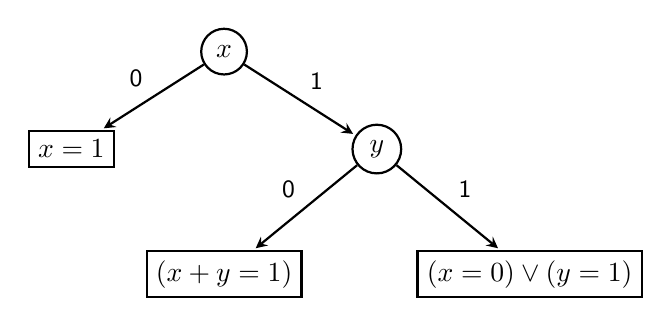
\begin{tikzpicture}[->,>=stealth,shorten >=1pt,auto,node distance=1.75cm, thick,main node/.style={scale=0.9,circle,draw,font=\sffamily\normalsize}]

        \node[circle, draw] (1)[] {$x$};

        \node[rectangle, draw] (2) [below left of=1, xshift=-20, ]{$x = 1$};
        \node[circle, draw] (3) [below right of=1, xshift=20, ]{$y$};

        \node[rectangle, draw] (4) [below left of=3, xshift=-20, yshift=-10]{$(x+y = 1)$};
        \node[rectangle, draw] (5) [below right of=3, xshift=20, yshift=-10]{$(x = 0) \lor (y = 1)$};

        \path[every node/.style={font=\sffamily\small}]
            (1) edge[swap]  node{0} (2)
            (1) edge node{1}(3)

            (3) edge[swap]  node{0} (4)
            (3) edge[]  node{1}(5)            
        ;
    \end{tikzpicture}

    \caption{The decision tree obtained from the proof of \Cref{treelike_proof}}
\end{figure}

\begin{lemma}
    Let $F$ be an linear CNF formula. If there is a PDT of size $s$ and depth $d$ that solves $S_F$, there also is a tree-like $\mathsf{TreeRes}_\oplus$ refutation of $F$ with size at most $2s$, depth at most $d+1$ and the weakening rule applied only to the leaves.
\end{lemma}

\begin{proof}
    Let $T$ be a PDT of size $s$ and depth $d$ that solved $S_F$. By \Cref{degenerate}, we assume that $T$ is non-degenerate. We label every node $v$ of $T$ with the negation of its associated linear system. In other words, every node $v$ is labeled with the linear clause $\lnot \Phi_v^T$. Clearly, every node is a result of the resolution rule being applied on it's children, where the root node is the empty clause.

    Since $T$ is a PDT that solves $S_F$, each leaf refutes a linear clause of $F$. Hence, for each leaf $u$ we have that $\Phi_{u}^T \implies \lnot C$ for some linear clause $C$ of $F$, which equivalently means that $C \implies \lnot \Phi_u^T$, concluding that the linear clause of each leaf is actually a weakening of a clause of $F$.
    
    Then, for each leaf $u$ we can add a new neighbor node $w$ and label it with the clause $C$, where the edge $(w,u)$ becomes an application of the weakening rule. This process increases the depth of the tree by 1 and increases the size by at most $s$.
\end{proof}

\begin{theorem}
    $\mathsf{FP}^{pdt}(S_F) = \Theta(\mathsf{TreeRes}_\oplus(F))$
\end{theorem}

\begin{proof}
    Follows from the two previous lemmas
\end{proof}

Itsykson and Sokolov showed that $\mathsf{TreeRes}_\oplus$ can efficiently simulate than $\mathsf{TreeRes}$ but the reverse doesn't hold \cite{res_lin_2}. This result also follows in a more natural way from our characterization since we showed $\mathsf{FP}^{dt} \subsetneq \mathsf{FP}^{pdt}$. In the same paper, they also discussed how $\mathsf{TreeRes}_\oplus$ cannot efficiently simulate regular resolution (or $\mathsf{RegRes}$), a restricted proof system derived from resolution. Due to any regular resolution also being a resolution proof, this result also implies that $\mathsf{TreeRes}_\oplus$ cannot efficiently simulate $\mathsf{Res}$. Thanks to \Cref{equiv_proof} and the fact that $\mathrm{PLS}^{dt}(S_F) = \Theta(\mathsf{Res}(F))$, we conclude the following black-box separation.

\begin{corollary}
    $\mathsf{FP}^{pdt} \neq \mathsf{PLS}^{dt}$
\end{corollary}

\section{Nullstallensatz over $\F_2$}

\section{$\mathrm{NS-}\F_2$ simulates $\mathrm{TreeRes}(\oplus)$}

\cleardoublepage